\documentclass[t,pdf]{beamer}
\mode<presentation>{}


\usecolortheme[RGB={196, 30, 58}]{structure}
\definecolor{lightgreen}{RGB}{ 220, 255, 220}
\definecolor{lightblue}{RGB}{ 220, 220, 255}

\usepackage{color}
\usepackage{animate}
\usepackage{tikz}
\usetikzlibrary{shadings,shadows}
\usetikzlibrary{shapes, arrows}
\usetikzlibrary{decorations.pathreplacing,angles,quotes}
\usetikzlibrary{calc}
\usetikzlibrary{positioning}
\usepackage{pgfplots}
\usepackage{booktabs,colortbl}
\usepackage{graphicx}

\usepackage{alltt}
\newenvironment{ccode}{\begin{alltt}\footnotesize}{\end{alltt}}


\usepackage{hyperref}
%% Colored hyperlink 
\newcommand{\cref}[2]{\href{#1}{\color{blue}#2}}
%% Colored hyperlink showing link in TT font
% \newcommand{\chref}[1]{\href{#1}{\small\tt \color{blue}#1}}
\newcommand{\hcref}[1]{\cref{#1}{\small\tt #1}}

\usepackage{booktabs,colortbl}

\newcommand{\keyword}[1]{\textbf{#1}}
\newcommand{\keyif}{\keyword{if}}
\newcommand{\keywhile}{\keyword{while}}
\newcommand{\keyfor}{\keyword{for}}
\newcommand{\keytrue}{\keyword{True}}
\newcommand{\keybreak}{\keyword{break}}
\newcommand{\keyreturn}{\keyword{return}}
\newcommand{\assign}{\ensuremath{\longleftarrow}}



\newcommand{\ground}{blue}
\definecolor{xred}{rgb}{0.77, 0.12, 0.23}
\definecolor{xgreen}{rgb}{0.3, 0.6, 0}
\definecolor{xblue}{rgb}{0., 0.25, 1}
\tikzstyle{grayfill} = [fill=fillcolor!70, draw=drawcolor, thick]
\tikzstyle{whitefill} = [fill=white, draw=drawcolor, thick] 
\definecolor{fillcolor}{rgb}{0.5, 0.5, 0.5} 
\definecolor{drawcolor}{rgb}{0, 0, 0} 

\definecolor{medgreen}{rgb}{0.34, 0.65, 0.34}
\definecolor{clearorange}{rgb}{0.917647, 0.462745, 0}
\definecolor{darkred}{rgb}{0.576471, 0.152941, 0.172549}


\definecolor{mediumgreen}{RGB}{20,140,20}
\definecolor{mediumblue}{RGB}{20,20,140}



\definecolor{bddneutralcolor}{RGB}{0,0,102}
\definecolor{bddpathcolor}{RGB}{25,25,255}
\definecolor{bddfillcolor}{RGB}{255,255,224}
\definecolor{bddbackground}{RGB}{230,240,255}
\definecolor{bddhighcolor}{RGB}{204,0,0}
\definecolor{bddlowcolor}{RGB}{0,143,0}

\definecolor{xred}{rgb}{0.77, 0.12, 0.23}
\definecolor{xgreen}{rgb}{0.3, 0.6, 0}
\definecolor{xblue}{rgb}{0., 0.25, 1}

\newcommand{\rtext}[1]{\textcolor{xred}{#1}}
\newcommand{\btext}[1]{\textcolor{xblue}{#1}}
\newcommand{\gtext}[1]{\textcolor{xgray}{#1}}

\newcommand{\showcomment}[1]{\rtext{\texttt{/*} \textit{#1} \texttt{*/}}}


\title{Trustworthy Boolean Reasoning \\ 2A: Introduction to BDDs}
%\subtitle{}
\author{Randal E. Bryant}


\institute{\includegraphics[height=50pt]{figs/CMU_Logo}}

\date{\textcolor{black}{June, 2022}}

\setbeamertemplate{footline}
{
	\leavevmode%
	\hbox{%
	\begin{beamercolorbox}[wd=0.35\paperwidth,ht=2.25ex,dp=1ex,center]{author in head/foot}%
	\tiny {Bryant: SSFT22}
			\vspace{4pt}
	\end{beamercolorbox}%
	\begin{beamercolorbox}[wd=0.45\paperwidth,ht=2.25ex,dp=1ex,center]{author in head/foot}%
	\end{beamercolorbox}%
	\begin{beamercolorbox}[wd=0.2\paperwidth,ht=2.5ex,dp=1ex,right]{date in head/foot}%
		\structure{\scriptsize \insertframenumber{} / \inserttotalframenumber\hspace*{3ex}}
		\vspace{3pt}
	\end{beamercolorbox}}%
	\vskip0pt%
}

\beamertemplatenavigationsymbolsempty

\begin{document}

\newcommand{\R}{\mathbb{R}}
\renewcommand{\P}{\mathbb{P}}
\newcommand{\E}{\mathbb{E}}
\newcommand{\Z}{\mathbb{Z}}
\newcommand{\N}{\mathbb{N}}
\newcommand{\diam}{\mbox{diam}}

\newcommand{\obar}[1]{\overline{#1}}
\newcommand{\anot}{\obar{a}}
\newcommand{\bnot}{\obar{b}}
\newcommand{\cnot}{\obar{c}}
\newcommand{\dnot}{\obar{d}}
\newcommand{\tnot}{\obar{t}}
\newcommand{\unot}{\obar{u}}
\newcommand{\vnot}{\obar{v}}
\newcommand{\wnot}{\obar{w}}
\newcommand{\xnot}{\obar{x}}
\newcommand{\znot}{\obar{z}}
\newcommand{\ite}{{\it ITE}}

\newcommand{\btrue}{1}
\newcommand{\bfalse}{0}

\newtheorem{conjecture}[theorem]{Conjecture}
\newtheorem{nonconj}[theorem]{(Not actually a) conjecture}


\AtBeginSection[]{
\begin{frame}{Table of Contents}
	\tableofcontents[currentsection]
\end{frame}
}

\begin{frame}
	\titlepage
\end{frame}




\frame{
  \frametitle{Important Ideas for These Lectures}
  \begin{itemize}
  \item SAT solvers are useful tools
    \begin{itemize}
    \item Many practical problems reducible to SAT
    \item Need to learn effective encoding techniques
    \end{itemize}
\medskip
  \item For many applications, formulas should be unsatisfiable
    \begin{itemize}
    \item Program should generate a checkable proof
    \item There is a well-developed proof infrastructure
    \end{itemize}

\medskip
  \item {\bf Binary Decision Diagrams (BDDs) can play important role}
    \begin{itemize}
    \item {\bf In supplementing current SAT algorithms}
    \item In proof generation
    \end{itemize}
  \end{itemize}
}


\frame{
\frametitle{Reduced Ordered Binary Decision Diagrams (BDDs)}

\begin{itemize}
\item Bryant, 1986
\item Based on earlier work by Lee (1959) and Akers (1978)  
\end{itemize}

{\bf Graph Representation of Boolean Functions}
\begin{itemize}
\item Canonical Form
\item Compact for many useful problems
\item Simple algorithms to construct \& manipulate
\end{itemize}

{\bf Used in SAT, Model Checking, $\ldots$}
\begin{itemize}
\item Bottom-up approach
  \begin{itemize}
  \item Construct canonical representation of problem
  \item Generate solutions
  \end{itemize}
\item Compare to search-based methods
  \begin{itemize}
  \item E.g., CDCL
  \item Top-down approaches
  \item Keep branching on variables until find solution
  \end{itemize}
\end{itemize}
}

\frame{
  \frametitle{Boolean Function Representations}

  \begin{minipage}[t]{0.35\textwidth}
    \begin{center}
    {\bf Truth Table}
    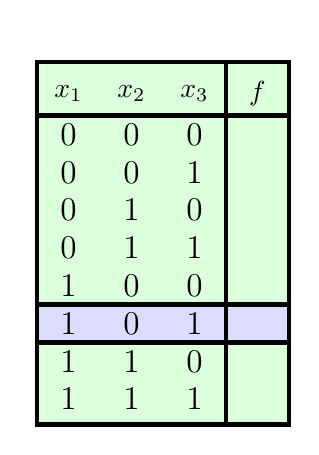
\begin{tikzpicture}[scale=4.0]
      %% Top boundary
      \node at (0.0,1.25) {};
      \draw[fill=lightgreen,ultra thick] (  0,  0.02) rectangle ( 0.80,  1.00);
      \draw[fill=lightgreen,ultra thick] (  0,  1.00) rectangle ( 0.80,  1.17);
      \draw[ultra thick] (0.60, 0.02) rectangle ( 0.80,  1.17);
      \only<2->{\draw[fill=lightblue,ultra thick] ( 0.0, 0.28) rectangle ( 0.80, 0.40);}
      \only<2->{\draw[fill=lightblue,ultra thick] ( 0.6, 0.28) rectangle ( 0.80, 0.40);}
      % Row 8
      \node at (0.10,0.10) {\large$1$};
      \node at (0.30,0.10) {\large$1$};
      \node at (0.50,0.10) {\large$1$};
      \node at (0.70,0.10) {\large$\btrue$};
      % Row 7
      \node at (0.10,0.22) {\large$1$};
      \node at (0.30,0.22) {\large$1$};
      \node at (0.50,0.22) {\large$0$};
      \node at (0.70,0.22) {\large$\bfalse$};
      % Row 6
      \node at (0.10,0.34) {\large$1$};
      \node at (0.30,0.34) {\large$0$};
      \node at (0.50,0.34) {\large$1$};
      \node at (0.70,0.34) {\large$\btrue$};
      % Row 5
      \node at (0.10,0.46) {\large$1$};
      \node at (0.30,0.46) {\large$0$};
      \node at (0.50,0.46) {\large$0$};
      \node at (0.70,0.46) {\large$\bfalse$};
      % Row 4
      \node at (0.10,0.58) {\large$0$};
      \node at (0.30,0.58) {\large$1$};
      \node at (0.50,0.58) {\large$1$};
      \node at (0.70,0.58) {\large$\btrue$};
      % Row 3
      \node at (0.10,0.70) {\large$0$};
      \node at (0.30,0.70) {\large$1$};
      \node at (0.50,0.70) {\large$0$};
      \node at (0.70,0.70) {\large$\bfalse$};
      % Row 2
      \node at (0.10,0.82) {\large$0$};
      \node at (0.30,0.82) {\large$0$};
      \node at (0.50,0.82) {\large$1$};
      \node at (0.70,0.82) {\large$\bfalse$};
      % Row 1
      \node at (0.10,0.94) {\large$0$};
      \node at (0.30,0.94) {\large$0$};
      \node at (0.50,0.94) {\large$0$};
      \node at (0.70,0.94) {\large$\bfalse$};
      % Headings
      \node at (0.10,1.07) {$x_1$};
      \node at (0.30,1.07) {$x_2$};
      \node at (0.50,1.07) {$x_3$};
      \node at (0.70,1.07) {$f$};
    \end{tikzpicture}
    \end{center}
  \end{minipage}%
  \begin{minipage}[t]{0.64\textwidth}
    \begin{center}
      {\bf Decision Tree}

      \input{bdd-dd/bdd-build-tree-path}
    \end{center}
  \end{minipage}
  
  \begin{itemize}
    \item Size $= O(2^n)$
    \only<2->{\item Assignment defines path from root to leaf}
  \end{itemize}
}

\frame{
  \frametitle{Reducing to Canonical Form}

  \begin{minipage}[t]{0.35\textwidth}
    \begin{center}
    {\bf Truth Table}
    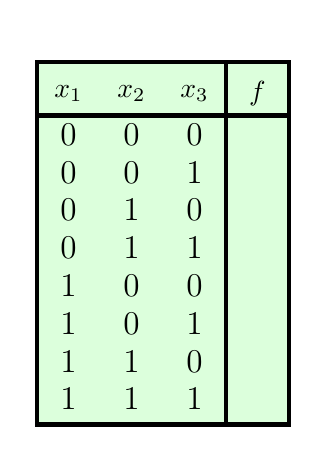
\begin{tikzpicture}[scale=4.0]
      %% Top boundary
      \node at (0.0,1.25) {};
      \draw[fill=lightgreen,ultra thick] (  0,  0.02) rectangle ( 0.80,  1.00);
      \draw[fill=lightgreen,ultra thick] (  0,  1.00) rectangle ( 0.80,  1.17);
      \draw[ultra thick] (0.60, 0.02) rectangle ( 0.80,  1.17);
      % Row 8
      \node at (0.10,0.10) {\large$1$};
      \node at (0.30,0.10) {\large$1$};
      \node at (0.50,0.10) {\large$1$};
      \node at (0.70,0.10) {\large$\btrue$};
      % Row 7
      \node at (0.10,0.22) {\large$1$};
      \node at (0.30,0.22) {\large$1$};
      \node at (0.50,0.22) {\large$0$};
      \node at (0.70,0.22) {\large$\bfalse$};
      % Row 6
      \node at (0.10,0.34) {\large$1$};
      \node at (0.30,0.34) {\large$0$};
      \node at (0.50,0.34) {\large$1$};
      \node at (0.70,0.34) {\large$\btrue$};
      % Row 5
      \node at (0.10,0.46) {\large$1$};
      \node at (0.30,0.46) {\large$0$};
      \node at (0.50,0.46) {\large$0$};
      \node at (0.70,0.46) {\large$\bfalse$};
      % Row 4
      \node at (0.10,0.58) {\large$0$};
      \node at (0.30,0.58) {\large$1$};
      \node at (0.50,0.58) {\large$1$};
      \node at (0.70,0.58) {\large$\btrue$};
      % Row 3
      \node at (0.10,0.70) {\large$0$};
      \node at (0.30,0.70) {\large$1$};
      \node at (0.50,0.70) {\large$0$};
      \node at (0.70,0.70) {\large$\bfalse$};
      % Row 2
      \node at (0.10,0.82) {\large$0$};
      \node at (0.30,0.82) {\large$0$};
      \node at (0.50,0.82) {\large$1$};
      \node at (0.70,0.82) {\large$\bfalse$};
      % Row 1
      \node at (0.10,0.94) {\large$0$};
      \node at (0.30,0.94) {\large$0$};
      \node at (0.50,0.94) {\large$0$};
      \node at (0.70,0.94) {\large$\bfalse$};
      % Headings
      \node at (0.10,1.07) {$x_1$};
      \node at (0.30,1.07) {$x_2$};
      \node at (0.50,1.07) {$x_3$};
      \node at (0.70,1.07) {$f$};
    \end{tikzpicture}
    \end{center}
  \end{minipage}%
  \begin{minipage}[t]{0.64\textwidth}
    \begin{center}
      {\bf Graph Representation}
      \only<1>{\input{bdd-dd/bdd-build-tree}}
      \only<2>{\input{bdd-dd/bdd-build-r4}}
      \only<3>{\input{bdd-dd/bdd-build-r3}}
      \only<4>{\input{bdd-dd/bdd-build-r2}}
    \end{center}
  \end{minipage}
  
  \begin{itemize}
    \item Merge isomorphic nodes
    \item Eliminate redundant tests
  \end{itemize}
}

\frame{
  \frametitle{Canonical Form}

  \begin{minipage}[t]{0.35\textwidth}
    \begin{center}
    {\bf Truth Table}
    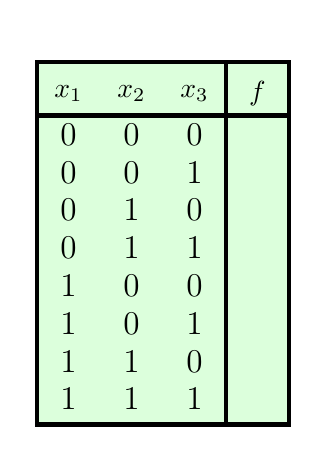
\begin{tikzpicture}[scale=4.0]
      %% Top boundary
      \node at (0.0,1.25) {};
      \draw[fill=lightgreen,ultra thick] (  0,  0.02) rectangle ( 0.80,  1.00);
      \draw[fill=lightgreen,ultra thick] (  0,  1.00) rectangle ( 0.80,  1.17);
      \draw[ultra thick] (0.60, 0.02) rectangle ( 0.80,  1.17);
      % Row 8
      \node at (0.10,0.10) {\large$1$};
      \node at (0.30,0.10) {\large$1$};
      \node at (0.50,0.10) {\large$1$};
      \node at (0.70,0.10) {\large$\btrue$};
      % Row 7
      \node at (0.10,0.22) {\large$1$};
      \node at (0.30,0.22) {\large$1$};
      \node at (0.50,0.22) {\large$0$};
      \node at (0.70,0.22) {\large$\bfalse$};
      % Row 6
      \node at (0.10,0.34) {\large$1$};
      \node at (0.30,0.34) {\large$0$};
      \node at (0.50,0.34) {\large$1$};
      \node at (0.70,0.34) {\large$\btrue$};
      % Row 5
      \node at (0.10,0.46) {\large$1$};
      \node at (0.30,0.46) {\large$0$};
      \node at (0.50,0.46) {\large$0$};
      \node at (0.70,0.46) {\large$\bfalse$};
      % Row 4
      \node at (0.10,0.58) {\large$0$};
      \node at (0.30,0.58) {\large$1$};
      \node at (0.50,0.58) {\large$1$};
      \node at (0.70,0.58) {\large$\btrue$};
      % Row 3
      \node at (0.10,0.70) {\large$0$};
      \node at (0.30,0.70) {\large$1$};
      \node at (0.50,0.70) {\large$0$};
      \node at (0.70,0.70) {\large$\bfalse$};
      % Row 2
      \node at (0.10,0.82) {\large$0$};
      \node at (0.30,0.82) {\large$0$};
      \node at (0.50,0.82) {\large$1$};
      \node at (0.70,0.82) {\large$\bfalse$};
      % Row 1
      \node at (0.10,0.94) {\large$0$};
      \node at (0.30,0.94) {\large$0$};
      \node at (0.50,0.94) {\large$0$};
      \node at (0.70,0.94) {\large$\bfalse$};
      % Headings
      \node at (0.10,1.07) {$x_1$};
      \node at (0.30,1.07) {$x_2$};
      \node at (0.50,1.07) {$x_3$};
      \node at (0.70,1.07) {$f$};
    \end{tikzpicture}
    \end{center}
  \end{minipage}%
  \begin{minipage}[t]{0.64\textwidth}
    \begin{center}
      {\bf Reduced Ordered \\ Binary Decision Diagram}
      \input{bdd-dd/bdd-build-canonical}
    \end{center}
  \end{minipage}
  
  \begin{itemize}
    \item Canonical representation of Boolean function
    \item No further simplifications possible
  \end{itemize}
}

\frame{
  \frametitle{BDD Representation of Unsatisfiable Formula}

\vskip 50pt

  \begin{center}
    \input{bdd-dd/zero}
  \end{center}

\vskip 30pt

  \begin{itemize}
  \item Refer to this as $\bot$
  \item Unique
  \item Converting from CNF to BDD may require exponential number of steps
  \end{itemize}

}


\frame{
  \frametitle{Effect of Variable Ordering}
\vskip -15pt

  $$(a_1 \land b_1) \lor (a_2 \land b_2) \lor (a_3 \land b_3)$$
  
  \begin{minipage}[t]{0.4\textwidth}
    \begin{center}
{\bf Good Ordering}    
    \input{bdd-dd/ordering-good}
    \begin{itemize}
      \item Linear growth
    \end{itemize}
    \end{center}
  \end{minipage} %
  \begin{minipage}[t]{0.55\textwidth}
    \begin{center}
    {\bf Bad Ordering}    
    \input{bdd-dd/ordering-bad}
    \begin{itemize}
      \item Exponential growth
    \end{itemize}
    \end{center}
  \end{minipage}
}

\frame{

  \frametitle{BDD Representation of Parity Constraints}
  \begin{minipage}{0.48\textwidth}
    \centering{
      Odd Parity\\[1.0em]
      \input{bdd-dd/parity-odd}
    }
  \end{minipage}
  \begin{minipage}{0.48\textwidth}
    \centering{
      Even Parity\\[1.0em]
      \input{bdd-dd/parity-even}
    }
  \end{minipage}

  \begin{itemize}
  \item Linear complexity
  \item Insensitive to variable order
  \item Potential major advantage over CDCL
  \end{itemize}
}

\frame{
\frametitle{Symbolic Manipulation with BDDs}

{\bf Strategy}
\begin{itemize}
\item Represent data as set of BDDs
  \begin{itemize}
    \item All with same variable ordering
  \end{itemize}
\item Express method as sequence of symbolic operations
  \begin{itemize}
    \item Generate new BDDs.  Test properties of BDDs
  \end{itemize}
\item Implement each operation via BDD manipulation
  \begin{itemize}
    \item Never enumerate individual cases
    \item Efficient, as long as BDDs stay small
  \end{itemize}
\end{itemize}
      
{\bf Key Algorithmic Properties}
\begin{itemize}  
  \item Arguments at each step are BDDs with same variable ordering
  \item Result is BDD with same ordering
  \item Each step has polymomial complexity
\end{itemize}
}

\frame{
  \frametitle{Apply Algorithm}
\begin{minipage}[t]{0.3\textwidth}
      \begin{eqnarray*} h & \leftarrow & f \odot g\end{eqnarray*}
\end{minipage}%
\begin{minipage}[t]{0.68\textwidth}
 \begin{itemize}
   \item $f$, $g$, $h$ functions represented as BDDs
   \item $\odot$ binary Boolean operator
     \begin{itemize}
     \item E.g., $\land$, $\lor$, $\oplus$
     \end{itemize}
 \end{itemize}
\end{minipage}


\begin{tikzpicture}
%% Top marker
  \node at (0,2.8) {};
  \node at (0,2.2) {$f$};
  \node at (0,0) {\includegraphics[scale=0.7]{bdd-dd/apply-argA-include}};
  \node at (1.8,0.6) {$\bigvee$};
  \node at (3.6,2.2) {$g$};
  \node at (3.6,0.0) {\includegraphics[scale=0.7]{bdd-dd/apply-argB-include}};
  \node at (5.4,0.6) {\huge $\rightarrow$};
  \node at (7.2,2.2) {$h = f \lor g$};
  \node at (7.2,0) {\includegraphics[scale=0.7]{bdd-dd/apply-result-include}};
\end{tikzpicture}

}

\frame{
  \frametitle{Apply Algorithm Recursion}
  \begin{itemize}
  \item Recurse through argument graphs
  \item Stop when hit terminal case
  \item Save results in cache to reuse when hit same arguments
  \end{itemize}

\begin{tikzpicture}
%% Top marker
  \node at (0,2.8) {};
  \node at (0,2.2) {$f$};
  \node at (0,0) {\includegraphics[scale=0.7]{bdd-dd/apply-argA-include}};
  \node at (3.0,2.2) {$g$};
  \node at (3.0,0.0) {\includegraphics[scale=0.7]{bdd-dd/apply-argB-include}};
  \node at (7.2,2.2) {Recursive Calls};
  \only<1>{\node at (7.2,-0.1) {\includegraphics[scale=0.7]{bdd-dd/apply-recurse-step1-include}};}
  \only<2>{\node at (7.2,-0.1) {\includegraphics[scale=0.7]{bdd-dd/apply-recurse-step2-include}};}
  \only<3>{\node at (7.2,-0.1) {\includegraphics[scale=0.7]{bdd-dd/apply-recurse-step3-include}};}
  \only<4>{\node at (7.2,-0.1) {\includegraphics[scale=0.7]{bdd-dd/apply-recurse-step4-include}};}
  \only<5>{\node at (7.2,-0.1) {\includegraphics[scale=0.7]{bdd-dd/apply-recurse-step5-include}};}
  \only<6>{\node at (7.2,-0.1) {\includegraphics[scale=0.7]{bdd-dd/apply-recurse-include}};}
\end{tikzpicture}

}


\frame{
  \frametitle{Apply Algorithm Result}

\begin{tikzpicture}
%% Top marker
  \node at (0,2.8) {};
  \node at (0,2.2) {Recursive Calls};
  \node at (0,-0.1) {\includegraphics[scale=0.7]{bdd-dd/apply-recurse-include}};
  \node at (5.0,2.2) {Reduced Result};
  \node at (5.0,0) {\includegraphics[scale=0.7]{bdd-dd/apply-result-include}};
\end{tikzpicture}

}

\begin{frame}

  \frametitle{BDD-Based SAT Solving: Direct Evaluation}



{\bf Algorithm}
\begin{enumerate}
\item    Compute BDD $t_i$ for each input clause $C_i$ 
\item    Form conjunction
  \begin{eqnarray*}
    s & = & \bigwedge_{1 \leq i \leq m} t_i
  \end{eqnarray*}
  \begin{itemize}
    \item E.g., with linear or tree evaluation
  \end{itemize}
\item Return UNSAT ($s = \bot$) or SAT ($s \not = \bot$)
\end{enumerate}


%%   \begin{tabbing}
%%     xxxxxx\=xxxx\=xxxx\=xxxx\=\kill
%%     \>$T \; \assign \;{} \emptyset$ \\
%%     \>\keyfor{} \; $C \in \{ C_1, C_2, \ldots, C_m \}$: \\
%%     \>\>$T \; \assign \; T \cup \{ {\it GenBDD}(C)\}$ \\
%%     \>\keywhile{} $|T| > 1$: \\
%%     \>\>Choose $s, t \in T$ \\
%%     \>\>$r \; \assign \;{\it ApplyAnd}(s, t)$\\
%%     \>\>\keyif{} $r = \bot$:\\
%%     \>\>\>\keyreturn{} UNSAT\\
%%     \>\>$T \; \assign{} \; T - \{s, t\} \cup \{r\}$\\
%%     \>Choose $t \in T$ \\
%%     \>\keyreturn{} SAT \\
%%   \end{tabbing}
%% 
%%   \vskip -10pt
{\bf Practicality}

  \begin{itemize}
  \item Only  for small problems
  \item Resulting BDD $s$ represents {\em all} solutions
  \end{itemize}

\end{frame}

\begin{frame}
\frametitle{Parity Benchmark Runtime}

\centering{%
\begin{tikzpicture}[scale = .80]
          \begin{axis}[mark options={scale=0.5},grid=both, grid style={black!10}, ymode=log, ymin=0.01, ymax=600.0, xmode=log, legend style={at={(0.95,0.35)}}, legend cell align={left},
                              x post scale=1.6,
                              ytick={0.01,0.1, 1.0, 10.0, 100.0, 600.0}, yticklabels={$0.01$,$0.1$,$1.0$,$10.0$,$100.0$,$600.0$},
                              xtick={10,100,1000,10000,100000}, xticklabels={$10$,$100$,$1{,}000$,$10{,}000$,$100{,}000$},xmin=10,xmax=100000,
            %%                  title={Parity Benchmark Runtime}
            ]
       \input{data-formatted/chew-kissat-seconds}
       \input{data-formatted/chew-tbsat-direct-seconds}
            \legend{
              \small \textsf{KISSAT},
              \small \textsf{TBSAT, Direct}
            }
          \end{axis}
\end{tikzpicture}
}

\begin{itemize}
\item TBSAT: BDD-Based SAT Solver
\item In direct mode, even worse than KISSAT
\item Limited to $n \leq 24$ within 600 seconds
\end{itemize}
\end{frame}


\begin{frame}

  \frametitle{BDD-Based SAT Solving: Bucket Elimination}

  \begin{itemize}
     \item Maintain list (``bucket'') $B_j$ for each variable $x_j$
     \item Each BDD stored in bucket according to root node variable
  \end{itemize}

{\bf Algorithm}
   \begin{tabbing}
     xxxxxx\=xxxx\=xxxx\=xxxx\=\kill
     \>{\em Initialization:} \\
    \>\>Form BDD $t_i$ for each input clause $C_i$ \\
    \>\>Place each $t_i$ in bucket according to ${\it Var}(t_i)$ \\
\\
  \>For each bucket $B_j$: \\
    \>\>Form conjunction $s_j$ of all BDDs in bucket $B_j$ \\
    \>\>If $s_j = \bot$ then return UNSAT \\
    \>\>Compute $r_j = \exists x_j s_j$ \\
    \>\>Place $r_j$ in bucket according to ${\it Var}(r_j)$ \\
\\
  \>return SAT \\
  \end{tabbing}

%%   
%%   \begin{tabbing}
%%     xxxxxx\=xxxx\=xxxx\=xxxx\=\kill
%%     \>$B_j \; \assign \;{} \emptyset$, $1 \leq j \leq n$ \\
%%     \>\keyfor{} \; $C \in \{ C_1, C_2, \ldots, C_m \}$: \\
%%     \>\>$t \; \assign \; {\it GenBDD}(C)$ \\
%%     \>\>$x_j \; \assign \; {\it Var}(t)$\\
%%     \>\>$B_j \; \assign \; B_j \cup \{ t \}$\\
%%     \>\keyfor{} \; $B \in \{ B_1, B_2, \ldots, B_n \}$: \\
%%     \>\>$s \; \assign \;{} {\it ApplyAndSet}(B)$ \\
%%     \>\>\keyif{} $s = \bot$:\\
%%     \>\>\>\keyreturn{} UNSAT\\
%%     \>\>$r \; \assign \;{} {\it ApplyOr}({\it High}(s), {\it Low}(s))$ \showcomment{Existential quant.}\\
%%     \>\>$x_k \; \assign \;{} {\it Var}(r)$\\
%%     \>\>$B_k \; \assign \; B_k \cup \{ r \}$\\
%%     \>\keyreturn{} SAT\\
%%   \end{tabbing}
%% 
%%   \vskip -20pt
%%   \begin{itemize}
%%   \item Existentially quantify variable at root of each bucket BDD $s$
%%   \item Finish with constant BDD $\bot$ or $\top$
%%   \end{itemize}

\end{frame}

\begin{frame}
\frametitle{Bucket Elimination Example}

\begin{centering}
  \only<1>{\input{bdd-dd/bucket-initial}}
  \only<2>{\input{bdd-dd/bucket-A-conjunct}}
  \only<3>{\input{bdd-dd/bucket-A-quant}}
  \only<4>{\input{bdd-dd/bucket-B-conjunct}}
  \only<5>{\input{bdd-dd/bucket-B-quant}}
  \only<6>{\input{bdd-dd/bucket-C-conjunct}}
\end{centering}
\begin{itemize}
  \only<1>{\item Initially: BDD for each input clause}
  \only<1>{\item In bucket according to root variable}
  \only<2>{\item Conjunct BDDs in topmost bucket $A$}
  \only<3>{\item Existentially quantify variable $a$}
  \only<3>{\item Place result in appropriate bucket}
  \only<4>{\item Conjunct BDDs in bucket $B$}
  \only<5>{\item Existentially quantify variable $b$}
  \only<5>{\item Place result in appropriate bucket}
  \only<6>{\item Conjunct BDDs in bucket $C$}
  \only<6>{\item Final result will be $\bot$ or $\top$}
\end{itemize}

\end{frame}




\begin{frame}
\frametitle{Parity Benchmark Runtime}

\centering{%
\begin{tikzpicture}[scale = .80]
          \begin{axis}[mark options={scale=0.5},grid=both, grid style={black!10}, ymode=log, ymin=0.01, ymax=600.0, xmode=log, legend style={at={(0.95,0.35)}}, legend cell align={left},
                              x post scale=1.6,
                              ytick={0.01,0.1, 1.0, 10.0, 100.0, 600.0}, yticklabels={$0.01$,$0.1$,$1.0$,$10.0$,$100.0$,$600.0$},
                              xtick={10,100,1000,10000,100000}, xticklabels={$10$,$100$,$1{,}000$,$10{,}000$,$100{,}000$},xmin=10,xmax=100000,
            %%                  title={Parity Benchmark Runtime}
            ]
       \input{data-formatted/chew-kissat-seconds}
       \input{data-formatted/chew-tbsat-direct-seconds}
       \input{data-formatted/chew-tbsat-bucket-seconds}
            \legend{
              \small \textsf{KISSAT},
              \small \textsf{TBSAT, Direct},
              \small \textsf{TBSAT, Bucket}
            }
          \end{axis}
\end{tikzpicture}
}

\begin{itemize}
\item $n=10{,}000$ in 633 seconds
\item Large benefit from quantification
\begin{itemize}
  \item abstracts away intermediate variables
\end{itemize}
\end{itemize}
\end{frame}

\begin{frame}

\frametitle{What Parity Benchmark Demonstrates}

\bigskip

\begin{itemize}
  \item Binary Decision Diagrams (BDDs) can play important role in SAT
    \begin{itemize}
    \item In supplementing current SAT algorithms
    \item But, {\em what about proof generation?}
    \end{itemize}
\end{itemize}


\end{frame}
  

\end{document}

%%% Local Variables:
%%% mode: latex
%%% TeX-master: t
%%% End:
